\begin{vbframe}{Linear Models -- Functionality}

% \maketag{SUPERVISED} 
\maketag{regression} \maketag{classification} \maketag{PARAMETRIC} 
\maketag{WHITE-BOX}
\medskip

\highlight{General idea} ~~ Represent target as function of linear predictor
$\thx$

\medskip

\highlight{Hypothesis space} ~~
$\Hspace = \left\{f: \Xspace \to \R ~|~\fx = \phi(\thetab^\top \xv)\right\}$, 
with suitable transformation $\phi(\cdot)$, e.g.,

\begin{itemize}
  \item Identity $\phi(\thetab^\top \xv) = \thetab^\top \xv$ 
  ~ $\Rightarrow$ \textbf{linear regression}
  % $\rightarrow$ continous output
  \item Logistic sigmoid function $\phi(\thx) = \frac{1}{1 + \exp(- \thx)} 
  =: \pixt$
  ~ $\Rightarrow$ \textbf{(binary) logistic regression}
  \begin{itemize}
    
    \item Probability $\pixt = \post$ of belonging to one of two classes
    \item Separating hyperplane via decision rule 
    (e.g., $\yh = 1 \Leftrightarrow \pix > 0.5$)
  \end{itemize}
\end{itemize}

\begin{minipage}[b]{0.32\textwidth}
  \begin{center}
    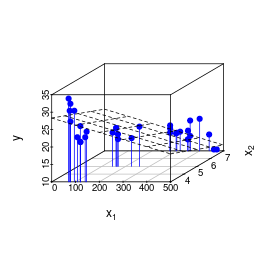
\includegraphics[width=0.9\textwidth, trim=0 40 0 0, clip]{
    figure/lm_3d.png} \\
    \tiny{Linear regression hyperplane}
  \end{center}
\end{minipage}
\begin{minipage}[b]{0.32\textwidth}
  \begin{center}
    % 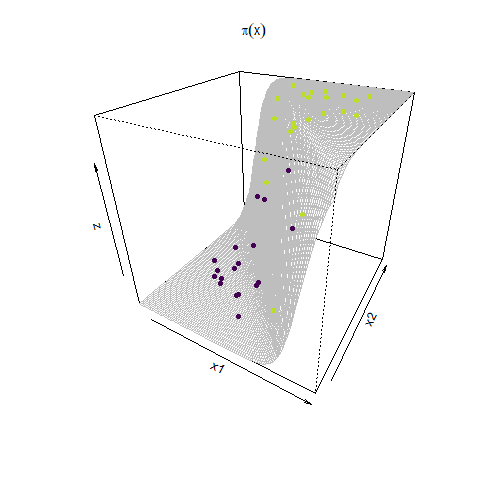
\includegraphics[width=0.7\textwidth, trim=0 40 0 0, clip]{
    % ../slides/supervised-classification/figure_man/logreg-2vars-surface}\\
    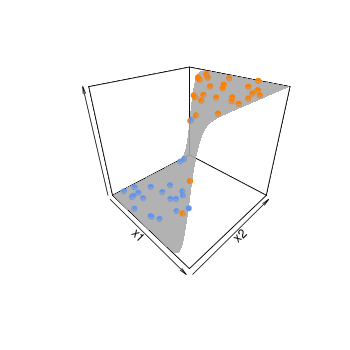
\includegraphics[width=0.7\textwidth, trim=30 50 0 0, clip]{figure/logreg_3d}\\
    \tiny{Logistic function for bivariate input and loss-minimal $\thetab$}
  \end{center}
\end{minipage}
\begin{minipage}[b]{0.32\textwidth}
  \begin{center}
    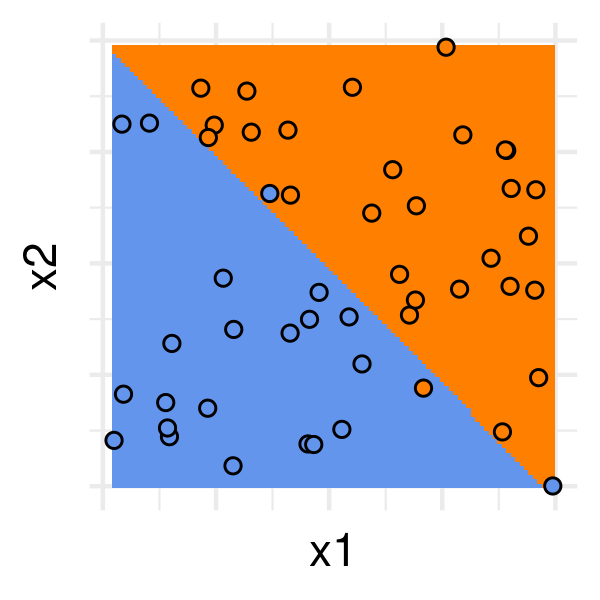
\includegraphics[width=0.5\textwidth]{figure/logreg_2d}\\
    % 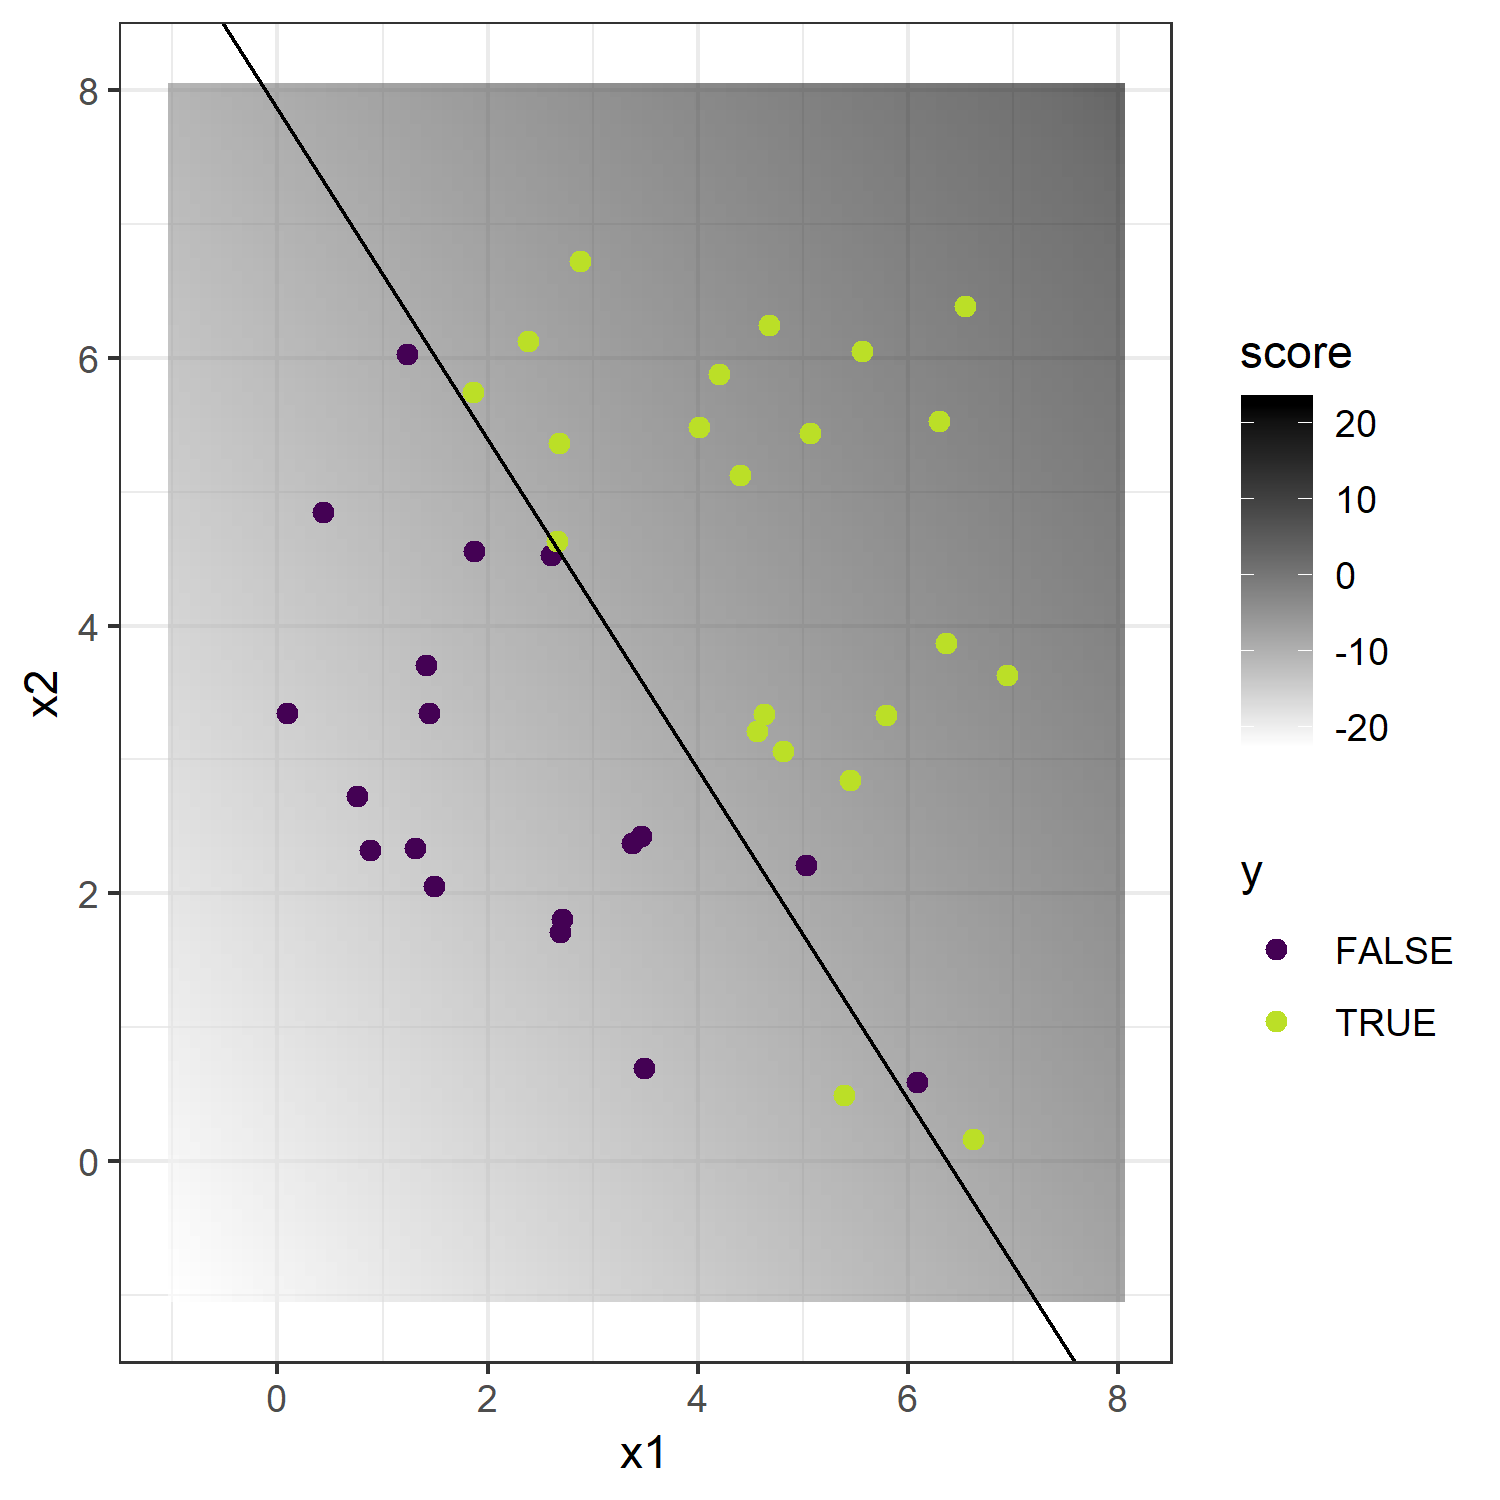
\includegraphics[width=0.6\textwidth]{
    % ../slides/supervised-classification/figure_man/logreg-2vars-data} \\
    \tiny{Corresponding separating hyperplane}
\end{center}
\end{minipage}

\framebreak

\highlight{Empirical risk}

\begin{itemize}
  \item \textbf{Linear regression}
  \begin{itemize}
    
    \item Typically, based on \textbf{quadratic} loss: $\risket = 
    \sumin \left(\yi - \fxit \right)^2$ \\
    $\Rightarrow$ corresponding to ordinary-least-squares (OLS) estimation
    \item Alternatives: e.g., \textbf{absolute} or \textbf{Huber} loss (both 
    improving robustness)
  \end{itemize}
  \item \textbf{Logistic regression:} based on 
  \textbf{Bernoulli/log/cross-entropy} loss ~ 
  $\Rightarrow \risket = \sumin -\yi \log 
  \left(\pixii\right) - (1 - \yi) \log \left(1 - \pixii \right)$
\end{itemize}

\medskip

\highlight{Optimization}
\begin{itemize}
  \item For \textbf{OLS}: analytically with 
  $\thetabh = \olsest$ \\
  (with $\Xmat \in \R^{n \times p}$ : matrix of feature vectors)
  \item For \textbf{other loss functions}: numerical optimization 
\end{itemize}

\medskip

\highlight{Hyperparameters} ~~ None

\medskip

% \highlight{Runtime behavior} ~~ $\mathcal{O}(p^2 \cdot n + p^3)$ for $n$ 
% observations and $p$ features

\end{vbframe}

% ------------------------------------------------------------------------------

\begin{frame}{Linear Models -- Pro's \& Con's}



\begin{columns}[onlytextwidth]
  \begin{column}{0.5\textwidth}
    \highlight{Advantages}
    
    \begin{itemize}
      \positem \textbf{Simple and fast} implementation
      \positem \textbf{Analytical} solution
      \positem \textbf{Cheap} computation
      \positem Applicable for any \textbf{dataset size}, as long as number of 
      observations $\gg$ number of features
      \positem Flexibility \textbf{beyond linearity} with polynomials, 
      trigonometric transformations etc.
      \positem Intuitive \textbf{interpretability} via feature effects
      % \positem fits \textbf{linearly} separable data sets very well
      \positem Statistical hypothesis \textbf{tests} for effects available

    \end{itemize}
  \end{column}

  \begin{column}{0.5\textwidth}
    \highlight{Disadvantages}
    
    \begin{itemize}
      \negitem \textbf{Nonlinearity} of many real-world problems
      \negitem Further restrictive \textbf{assumptions}: linearly independent 
      features, homoskedastic residuals, normality of conditional response
      \negitem \textbf{Sensitivity} w.r.t. outliers and noisy data (especially 
      with L2 loss)
      \negitem Risk of \textbf{overfitting} in higher dimensions
      \negitem Reature \textbf{interactions} must be handcrafted, so higher
      orders practically infeasible
      \negitem No handling of \textbf{missing} data
    \end{itemize}
  \end{column}
\end{columns}

\vfill

\small

\conclbox{Simple, highly interpretable method suited for linear problems, but 
with strong assumptions,\\ practical limitations, and tendency to overfit}

\end{frame}

% ------------------------------------------------------------------------------

\begin{frame}{Linear Models -- regularization}

\highlight{Idea}

\begin{itemize}
  \item Unregularized LM: risk of \textbf{overfitting} in high-dimensional 
  space with only few observations
  \item \textbf{Goal}: find compromise between model fit and generalization by 
  adding \textbf{penalty term}
\end{itemize}

\medskip

% \highlight{Hypothesis space} ~~\\
% $\Hspace = \left\{f: \Xspace \to \R ~|~\fx = \phi(\thetab^\top \xv)\right\}$, 
% where $\phi(\cdot)$ is a transformation function.


%$\Hspace = \{ \theta_0 + \thx\ |\ (\theta_0, \thetab) \in \R^{p+1} \} $

\medskip

\highlight{Regularized empirical risk}

\begin{itemize}
  \item Empirical risk function \textbf{plus complexity penalty} 
  $J(\thetab)$, controlled by shrinkage parameter $\lambda > 0$: \\
  $\riskrt := \risket + \lambda \cdot J(\thetab).$ 
  \item Popular regularizers
  \begin{itemize} 
    \item \textbf{Ridge} regression: L2 penalty $J(\thetab) = \|\thetab\|_2^2 $
    \item \textbf{LASSO} regression: L1 penalty $J(\thetab) = \|\thetab\|_1 $
  \end{itemize}
\end{itemize}

\medskip

\highlight{Optimization under regularization}
\begin{itemize}
  \item \textbf{Ridge}: analytically with 
  $\thetabh_{\text{Ridge}} = (\Xmat^\top \Xmat  + \lambda \id)^{-1} \Xmat^\top 
  \yv$
  \item \textbf{LASSO}: numerically with, e.g., (sub-)gradient descent
\end{itemize}

\end{frame}

% ------------------------------------------------------------------------------

\begin{frame}{Linear Models -- regularization}

\highlight{Choice of regularization parameter}

\begin{itemize}
  \item Standard hyperparameter optimization problem
  \item E.g., choose $\lambda$ with minimum mean cross-validated error 
  (default in R package \texttt{glmnet})
\end{itemize}

\medskip

\highlight{Ridge vs. LASSO} 

\begin{itemize}
  \item \textbf{Ridge}
  \begin{itemize} 
    \item Overall smaller, but still dense $\thetab$
    \item Suitable with many influential features present, handling correlated 
    features by shrinking their coefficients equally
  \end{itemize}
  \item \textbf{LASSO}
  \begin{itemize} 
    \item Actual variable selection
    \item Suitable for sparse problems, ineffective with correlated 
    features (randomly selecting one)
  \end{itemize}  
  \item Neither overall better -- compromise: \textbf{elastic net} \\
  $\rightarrow$ weighted 
  combination of Ridge and LASSO regularizers
\end{itemize}


\end{frame}

% ------------------------------------------------------------------------------

\begin{frame}{Linear Models -- Practical hints}

\highlight{Implementation}

\begin{itemize}
  \item \textbf{R:}
  \begin{itemize}
    \item \textbf{Unregularized:} \texttt{mlr3} learner \texttt{LearnerRegrLM}, 
    calling \texttt{stats::lm()} / \texttt{mlr3} learner 
    \texttt{LearnerClassifLogReg}, calling \texttt{stats::glm()}
    \item \textbf{Regularized:} \texttt{mlr3} learners 
    \texttt{LearnerClassifGlmnet} / 
    \texttt{LearnerRegrGlmnet}, calling \texttt{glmnet::glmnet()}
  \end{itemize}
  \item \textbf{Python:} \texttt{LinearRegression} from package 
  \texttt{sklearn.linear\_model}, package for advanced statistical parameters 
  \texttt{statsmodels.api} 
\end{itemize}

%% WOULD DELTETE THIS!
%  \highlight{\textcolor{blue}{Check assumptions??} }\\
% Linear models are effective if the following assumptions are fulfilled:
%  \begin{itemize}
%   \item \textbf{linearity}: The expected response is a linear combination of the features.
%   \item \textbf{homoscedasticity}: The variance of residuals is equal for all features.
%   \item \textbf{independence}: All observations are independent of each other.
%   \item \textbf{normality}: Y is normally distributed for any fixed value of the features
% \end{itemize}

\end{frame}